\documentclass{beamer}




\usepackage{graphicx}
\usepackage{subfigure}
\usepackage{amssymb}
\usepackage{amsmath}
\usepackage{booktabs}
\usepackage{subfigure,pgf,tikz}
\usetikzlibrary{arrows}
\usepackage[misc]{ifsym}
\usepackage{mathrsfs}
\usepackage{epstopdf}


\usepackage{graphicx,xcolor,subfigure}

\usepackage{xeCJK}

\setCJKmainfont{微軟正黑體}

\XeTeXlinebreaklocale "zh"

\XeTeXlinebreakskip = 0pt plus 1pt


\usetheme{Boadilla}

\setbeamertemplate{footlines}[page number]{}
\setbeamertemplate{navigation symbols}

\title[]{}

\author[]{ }



\date[]{}

\setbeamertemplate{theorems}[numbered]

\theoremstyle{plain}
\newtheorem{thm}{Theorem}[section]
\newtheorem{cor}[thm]{Corollary}
\newtheorem{lem}[thm]{Lemma}
\newtheorem{prop}[thm]{Proposition}





\theoremstyle{definition}
\newtheorem{ex}[thm]{Exercise}
\newtheorem{defn}[thm]{Definition}
\newtheorem{prob}[thm]{Problem}
\newtheorem{exam}[thm]{Example}
\newtheorem{rem}[thm]{Remark}
\newtheorem{ques}[thm]{Question}
\newtheorem{conj}[thm]{Conjecture}

\begin{document}




\begin{frame}{\bf Definitions}


\begin{enumerate}
\item A \textcolor{red}{\bf triangulated graph} is a planar graph such that any edge is in a face and any face is a triangle.
\item A \textcolor{red}{\bf chordal graph} is a graph such that every cycle of length at least $4$ contains a \textcolor{red}{\bf chord}, i.e., an edge connecting two nonadjacent vertices of the cycle.
\item Is a triangulated graph a chordal graph?
\item A \textcolor{red}{\bf weakly  pancyclic graph} is a graph which contains cycles of every length between the girth and the circumference.
\item A graph is \textcolor{red}{\bf $t$-tough}  if for every integer $k>1$, the graph cannot be split into $k$ components by removal of fewer than $tk$ vertices
\item Hence a $t$-tough graph with $t>0$ is connected.
\end{enumerate}

\end{frame}









\begin{frame}{\bf Conjectures}

\begin{enumerate}
\item A triangulated graph is weakly  pancyclic.
\item A chordal graph is weakly  pancyclic.
\item There is a  $9$-tough triangulated non-Hamiltonian graph.
\item A $9.1$-tough triangulated graph is Hamiltonian.
\end{enumerate}
\bigskip



[1] Adam Kabela, Tom\'{a}\v{s} Kaiser, $10$-tough chordal graphs are Hamiltonian, Journal of Combinatorial Theory, Series B, Volume 122, January 2017, Pages 417-427.
\end{frame}


\begin{frame}{\bf Locally property $P$}

Let $P$ be a property on graphs.
A graph $G$ has \textcolor{red}{\bf local $P$} if $G_1(v)$ has property $P$ for every vertex $v$ in $G$.
\bigskip


Hence a triangulated graph is locally connected.
\end{frame}

\begin{frame}{\bf Lemma}
If $G$ is $1$-tough and locally $1$-tough then $G-u$ is $1$-tough for every vertex $u$ in $G$.

\begin{proof}
Assume that $G-u$ is split into $k$ components by removal fewer than $k$ vertices, and $t$ of these components intersect $G_1(u)$.
Then among the $k$ removal vertices there are at least $t$ from $G_1(u)$ and the remaining at most $k-t$ from $G-u-G_1(u)$ since $G_1(u)$ is $1$-tough.
Then $G$ is split into $1+(k-t)$ components by  by removal fewer than $1+k-t$ vertices in $G-G_1(u)$, a contradiction to the $1$-tough assumption of $G$.
\end{proof}
\end{frame}


\begin{frame}{\bf A $1$-tough and locally $1$-tough graph}
\begin{center}
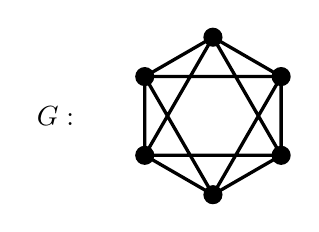
\begin{tikzpicture}[scale=1]

\foreach \i in {0,1,...,5}
{
\coordinate (v\i) at ({sin(2*\i*pi /6 r)},{cos(2*\i*pi /6 r)}) ;
}


\draw[very thick] (v4)--(v2)--(v0)--(v1)--(v2)--(v3)--(v4)--(v5)--(v0)--(v4) (v5)--(v3)--(v1)--(v5) ;
\draw[very thick,fill] (v0) circle (.1);
\draw[very thick,fill] (v1) circle (.1);
\draw[very thick,fill] (v2) circle (.1);
\draw[very thick,fill] (v3) circle (.1);
\draw[very thick,fill] (v4) circle (.1);
\draw[very thick,fill] (v5) circle (.1);
\draw(-2,0) node {$G:$};
\end{tikzpicture}
\end{center}
\end{frame}

\begin{frame}{\bf More conjectures}
\begin{enumerate}
\item  A $1$-tough and locally $1$-tough graph is weakly pancyclic.
\item  A $1$-tough and locally $1$-tough graph is Hamiltonian.
\end{enumerate}

\end{frame}
\end{document} 